\documentclass[12pt]{article}

%-----------------------------------------------------------%
%-------------TEST POUR LA FICHE DE SYNTHESE----------------%
%-----------------------------------------------------------%

\usepackage{geometry}
\usepackage{lipsum}
\usepackage{xcolor}
\usepackage{graphicx}
\usepackage{amsmath}

\pagestyle{empty}
\geometry{a4paper}
\geometry{top=0.5cm, bottom=2cm, left=1cm, right=1cm}

\begin{document}
\parindent=0pt

%Debut de l'entete------------------------------------------%
%------------------Les logos--------------------------------%
\begin{minipage}{0.55\linewidth}
    \begin{flushleft}
    
\includegraphics[scale=0.28]{ESRF_logo.png}
    \end{flushleft}
\end{minipage}
\hfill
\begin{minipage}{0.40\linewidth}
    \begin{center}
    
\includegraphics[scale=0.28]{logo-lille1-2014.png}
    \end{center}
\end{minipage}

\vspace{0.2cm}
\hrulefill
\vspace{0.2cm}

%------------------Bloc de gauche---------------------------%
\begin{minipage}{0.25\linewidth}
    \begin{center}
    \textbf{Guillaume Bonamis}\\
    \textbf{Master 1 Physique}\\ %en francais ou en anglais ???
    \textbf{2014-2015}
    \end{center}
\end{minipage}
%------------------Bloc du centre---------------------------%
\hfill
\begin{minipage}{0.30\linewidth}
    \begin{center} 
    \textbf{Universit\'e Lille 1}\\
    \textbf{UFR de Physique}\\

    Tutor: Emeline Dudognon
    \end{center}
\end{minipage}
%------------------Bloc de droite---------------------------%
\hfill
\begin{minipage}{0.30\linewidth}
    \begin{center}
    \textbf{ESRF}\\
    \textbf{Data Analysis Unit}\\

    Supervisor: J\'er\^ome Kiffer
    \end{center}
\end{minipage}
%Fin de l'entete--------------------------------------------%


%Intitule du stage------------------------------------------%
\begin{center}
    \fbox{\begin{minipage}{\linewidth}
    \begin{center}\bfseries\Huge 
        Modeling of the shape of proteins from SAXS data
    \end{center}
    \end{minipage}}
\end{center}
%-----------------------------------------------------------%


%Introduction du sujet--------------------------------------%
\begin{center}%Il faudra surement faire plus court, plus rentre dedans
\fbox{\begin{minipage}{\linewidth}
    \textbf{SAXS}: 
    Small Angles X-ray Scattering experiments of biological macromolecule 
    solutions at the BioSAXS beamline BM29 at the ESRF aim at determining 
    their 3-dimensional structures in a natural state with a ’low’ 
    resolution, a few nm.
    SAXS experiment provides a 2-dimensional scattering image. 
    Using the cylindrical symmetry along the transmitted beam, an 
    azimuthal integration and a background correction are performed to 
    obtain the scattering curve of the sample. 
    This curve is the starting point of the modeling process.
\end{minipage}}
\end{center}
%-----------------------------------------------------------%

\vspace{-0.6cm}
%------bloc texte a gauche, image a droite------------------%
\begin{minipage}{0.60\linewidth}
    \begin{center}\begin{large}
    scattering curve$\overset{\textit{dammif}}{\longrightarrow}$dummy-atoms models (DAM)
    \end{large}\end{center}
    An exemple of DAM is presented on right side (lysozyme).\\
    To compute a reliable 3-d model of the protein, this process has to 
    be launched several time and "averaged". 
    We wrote \textbf{FreeSAS}, a Python package to do a part of this work.
\end{minipage} \hfill
\begin{minipage}{0.35\linewidth}
    \begin{flushleft}
    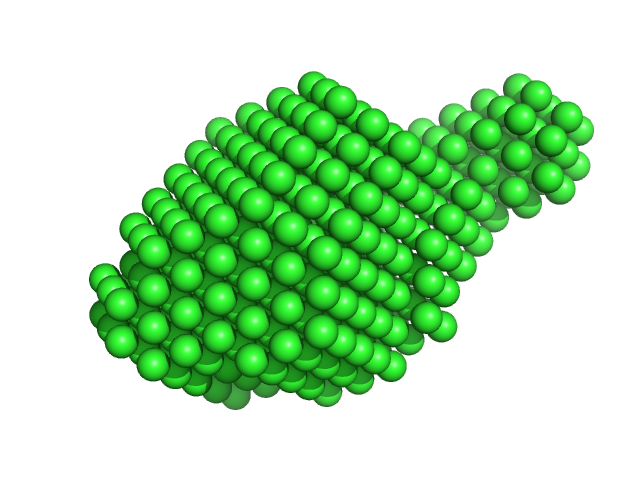
\includegraphics[scale=0.3]{model.png}
    \end{flushleft}
\end{minipage}
%-----------------------------------------------------------%

\vspace{-0.5cm}
%------bloc texte a droite, image a gauche------------------%
\begin{minipage}{0.35\linewidth}
    \begin{flushleft}
    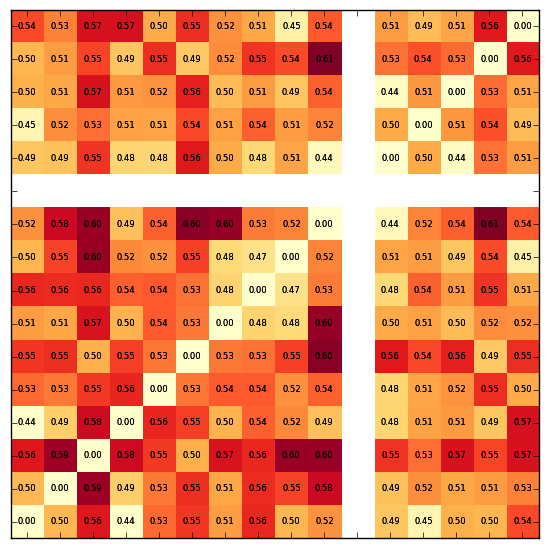
\includegraphics[scale=0.45]{nsdtable.png}
    \end{flushleft}
\end{minipage} \hfill
\begin{minipage}{0.60\linewidth}
    \begin{large}
    16 dammif ran $\longrightarrow$ 16 DAM ramdomly oriented
    \end{large}\\
    First, a selection by goodness of fit (SAXS curve) is performed.\\
    Then FreeSAS measures the similarity between each models using the 
    Normalized Spatial Discrepancy (NSD, Kozin and Svergun).\\
    DAM are first superimposed using a translation and a rotation. 
    Translation superimposes the center of mass of both models and the 
    rotation aligns their principle axis of inertia.\\
    After alignment, NSD are calculated and a 16*16 NSD table is 
    computed (on the left).
\end{minipage}
%-----------------------------------------------------------%

\vspace{-0.5cm}
%------bloc texte a gauche, image a droite------------------%
\begin{minipage}{0.55\linewidth}
    Most dis-similar models (by NSD) are discarded for the rest of the 
    BM 29 pipeline.\\
    Valid models are superimposed and their dummy-atoms coordinates are 
    saved. 
    Valid models among 16 \textit{dammif} models of lysozyme are 
    presented on the right.
\end{minipage} \hfill
\begin{minipage}{0.4\linewidth}
    \begin{flushleft}
    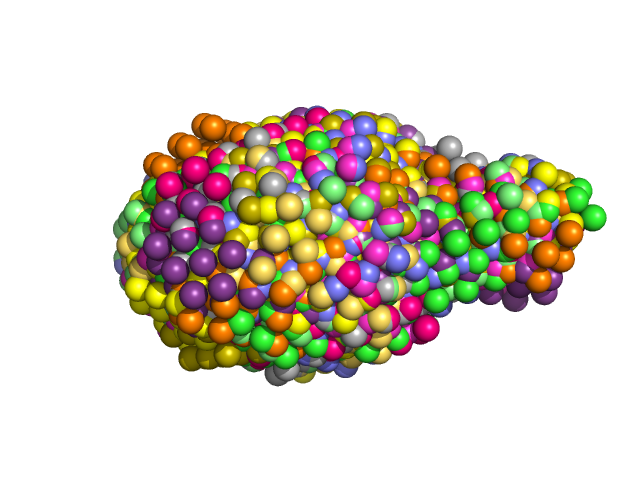
\includegraphics[scale=0.3]{validmodels.png}
    \end{flushleft}
\end{minipage}
%-----------------------------------------------------------%


%Notes de fin-----------------------------------------------%
\begin{center}
\fbox{\begin{minipage}{\linewidth}
\begin{minipage}{0.70\linewidth}
    reference: Kozin and Svergun, \textit{Journal of Applied Crystallography, 2001}
\end{minipage}
\hfill
\begin{minipage}{0.25\linewidth}
    
\end{minipage}

\begin{minipage}{0.95\linewidth}
    \textbf{Keywords}: 
    SAXS, structural modeling, Python 
\end{minipage}
\end{minipage}
}
\end{center}
%-----------------------------------------------------------%
\end{document}
